\chapter{Alternative Ansätze}
\label{Alternative Ansätze}

Nicht jeder Entwickler möchte in dem von ihm gewählten Backend auf CouchDB setzten müssen. Seien es persönliche Vorlieben oder technische Gegebenheiten, die eine alternative Datenbank für sinnvoller erscheinen lassen, kann trotzdem noch auf die Synchronisationsfeatures von PouchDB zurückgegriffen werden. So können beispielsweise auch von den großen Cloud-Anbietern (Amazon und Microsoft) angebotene Produkte zur Datenhaltung mit PouchDB auf den Endgeräten verknüpft werden. Im folgenden Kapitel wird beispielhaft erläutert, wie die Implementierung von PouchDB unter Verwendung einer SQL-Lite Datenbank aussehen kann und auf weitere Alternativen eingegangen.

\section{PouchDB als SQL-Lite Sync-API}
Bei der Verwendung von PouchDB als Technologie zur Synchronisation verschiedener Datenbestände mit einem gemeinsamen Backend nimmt CouchDB als Backend-Datenbank eine Sonderrolle ein. Da PouchDB das \emph{CouchDB replication protocol} implementiert \cite{pouch:syncnoncouchdb}, können Instanzen dieser No-SQL Datenbank direkt angesprochen werden, vergleichbar mit der Verwendung eines OR-Mappers welcher direkt auf einen SQL-Server zugreift. Für die Verwendung einer anderen Backend-DB, in diesem Beispiel SQL-Lite, müssen daher Änderungen auf Seiten des Backends in Kauf genommen werden. Da SQL-Lite selbst das zuvor genannte, von CouchDB vorgegebene Replikationsprotokoll nicht implementiert, muss eine entsprechende Komponente vorgeschalten werden, welche die ankommenden Requests in SQL-Lite kompatible Statements umwandelt.

Dies kann erreicht werden, indem das Backend vergleichbar mit einem weiteren Synchronisationsteilnehmer auf Basis von Node.js selbst das PouchDB-Paket nutzt, dieses aber entgegen der Endgeräte um einen SQL-Lite Adapter ergänzt \cite{pouch:sqlliteplugin}. Um die Implementierung eines solchen Backendservers zu erleichtern stellen die Entwickler von PouchDB für diese Zwecke über GitHub ein entsprechendes Repository bereit \cite{pouch:pouchdbserver}.

\begin{figure}[htb]
	\centering
	\caption{Schema der Architektur unter Nutzung eines PouchDB-Adapters für die Synchronisation mit einer SQL-Lite Instanz}
	\label{fig:pouchdbadapter}
	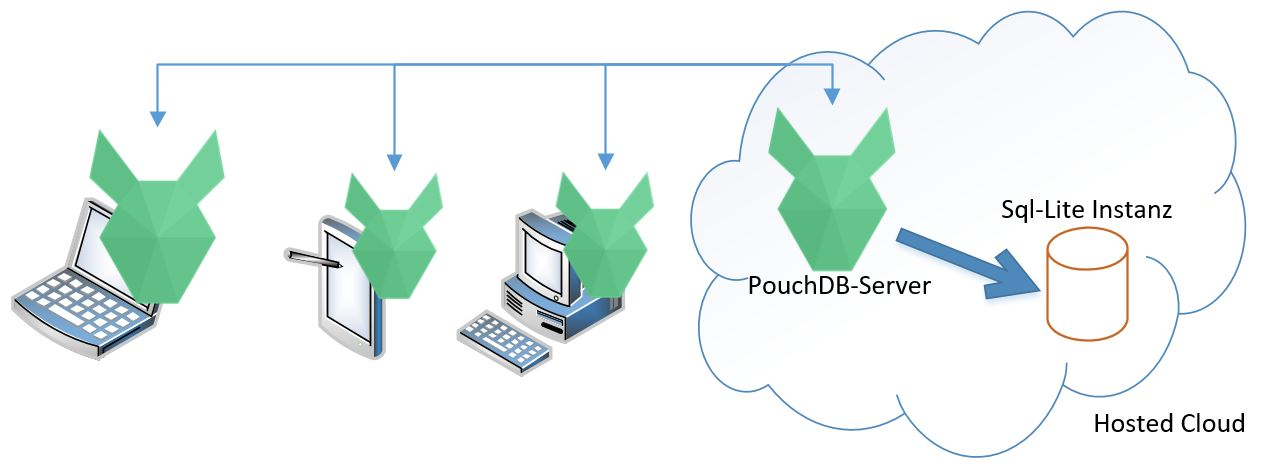
\includegraphics[width=\textwidth]{\figdir/PouchDbAltBackendDb.JPG}
\end{figure}

Für Entwickler, welche die SQL-Lite Instanzen auf eigenen Servern hosten bedeutet dies, dass durch eine Installation von Node.js für die Anbindung an die PouchDB-Kommunikation eine volle Synchronisation erreicht werden kann. Ob diese beiden Komponenten allerdings auf der gleichen (virtuellen) Maschine gehostet werden sollten, liegt im eigenen Ermessen. Werden die Datenbank-Instanzen hingegen als Software-as-a-Service von großen Cloud-Providern gemietet, bedeutet die Notwendigkeit eines PouchDB-Syncadapters allerdings, entweder weitere Ressourcen (Webserver/Node.js-Host) mieten zu müssen, oder ein anderes Verfahren für die Datensynchronisation zu nutzen.

\section{Alternativen zum CouchDB Replication Protocol}
Um die Eignung alternativer Technologien beurteilen zu können müssen die Key-Features von PouchDB als Kriterien herangezogen werden. Konkurrenten sollten ebenfalls die Möglichkeit bieten, Daten auch offline vorhalten zu können, sowie eine Synchronisation über mehrere Geräte und einem Backend ermöglichen. Darüber hinaus sollte eine mit PouchDB vergleichbare Kompatibilität gegeben sein, das heißt die Technologie sollte sich sowohl für die Mobil- als auch Webentwicklung nutzen lassen.

\subsection{Firebase by Google}
Einer der offensichtlichsten, wenn auch vom Feature-Umfang klar überlegen Mitbewerber ist die Tool-Sammlung Firebase von Google \cite{google:firebase}. Ursprünglich eine synchronisierende Cloud-Datenbank, wurde unter dem bekannten Namen inzwischen eine ganze Suite von Tools für die App-Entwicklung gesammelt, welche es Entwicklern erlauben soll, alle notwendigen Dienste aus einem Paket beziehen zu können. Darunter befinden sich auch interessante Features wie Reporting und Advertising-Komponenten. Hinsichtlich der gegebene Kriterien für PouchDB-Alternativen bietet Firebase alle notwendigen Eigenschaften. Die Daten können auf den jeweiligen Geräte offline bereitgestellt und bei bestehender Verbindung synchronisiert werden \cite{google:offlinejs}\cite{google:offlineandroid}. Außerdem kann das Toolset sowohl für android-native Applikationen als auch allgemein als JavaScript-Paket verwendet werden, was die Bedingungen hinsichtlich Kompatibilität ebenfalls erfüllt. Ein gegenüber von PouchDB allerdings bestehender Nachteil ist, dass das Backend zwangsweise von Google gestellt und daher gemietet werden muss. Wie für Cloud-Komponenten üblich erfolgt die Bezahlung zwar nach dem pay-as-you-go Prinzip, trotzdem verliert der Entwickler in diesem Punkt einige Freiheiten.

\subsection{Realm Mobile Database}
Ein weiterer Konkurrent auf dem Markt für synchronisierende Datenbestände in mobilen Applikationen ist Realm.io. Das nach eigenen Angaben mit knapp 30 Millionen Dollar unterstützte Unternehmen schreibt auf der eigenen Website von über einer Milliarde Installationen \cite{realm:about}, womit es zu den eher größeren Spielern auf dem Markt zählt. Die Angebotenen Produkte beinhalten eine Mobile-Platform, welche die Integration in Apps und Websiten erlaubt sowie die Synchronisation der auch offline verfügbaren Daten. Dabei setzt Realm auf eine Open-Source Datenbank, welche wie auch größte Teile des sonstigen Codes auf GitHub zu Verfügung steht \cite{realm:githubrepo}. Die Kompatibilität ist durch eine JavaScript-Implementierung mit der von PouchDB vergleichbar, Entwickler bestimmter Plattformen freuen sich aber auch über dedizierte Bibliotheken, beispielsweise für die Sprachen C++ oder Swift. Leider gibt die auf der Website verfügbare Kostenaufstellung wenig über die tatsächlichen Kosten preis, lediglich für die Business-Variante wird verraten, dass mindestens 1.500\$ im Monat berechnet werden.

\subsection{Microsoft Azure Mobile Apps}
Als letzte hier genannte Alternative sollte Microsofts \emph{Azure Mobile Apps}-Programm genannt werden. Im Gegensatz zu den vorherrschenden Meinungen hat sich das Unternehmen in den vergangenen Jahren mehr und mehr anderen Plattformen gegenüber geöffnet und möchte mit der eigenen Azure-Cloud mobile Entwicklung für alle Betriebssysteme ermöglichen.
Microsoft bietet daher auch die Möglichkeit, in Zusammenarbeit mit den eigenen Cloudspeicher-Varianten Daten offline auf mobilen Geräten bereit zu stellen und bei bestehender Internetverbindung zu synchronisieren \cite{microsoft:azuremobileappssync}. Im Gegensatz zu den beiden vorhergehenden Möglichkeiten kann hier aber auf keine JavaScript-Implementierung zurückgegriffen werden. Microsoft bietet die Bibliotheken bisher nur nativ für die einzelne Plattformen (iOS, Android, Windows) und für die inzwischen eingekaufte Cross-Compilerlösung Xamarin an.
